\documentclass{article}
\usepackage{fancyhdr}
\usepackage{lastpage}
\usepackage{amsmath}
\usepackage{amssymb}
\usepackage{amsthm}
\usepackage[margin=1in]{geometry}
\usepackage{graphicx}
\graphicspath{ {./} }

\pagestyle{fancy}
\setlength\headheight{28pt}
\addtolength{\headheight}{\baselineskip}
\fancyhf{}
\renewcommand{\headrulewidth}{0pt}
\lhead{Math 251 - Shuichi Masuda\\Juno Suárez\\\today}
\rfoot{Page \thepage \hspace{1pt} of \pageref{LastPage}}

\renewcommand\thesubsection{\arabic{subsection}.}
\renewcommand\thesubsubsection{\alph{subsubsection})}

\begin{document}

\section*{Computer Lab \# 4}

\renewcommand\thesubsection{1 - 9.}
\subsection{}
\emph{Steps performed in GeoGebra.}
\\
\\
\textbf{\# 8.} \\
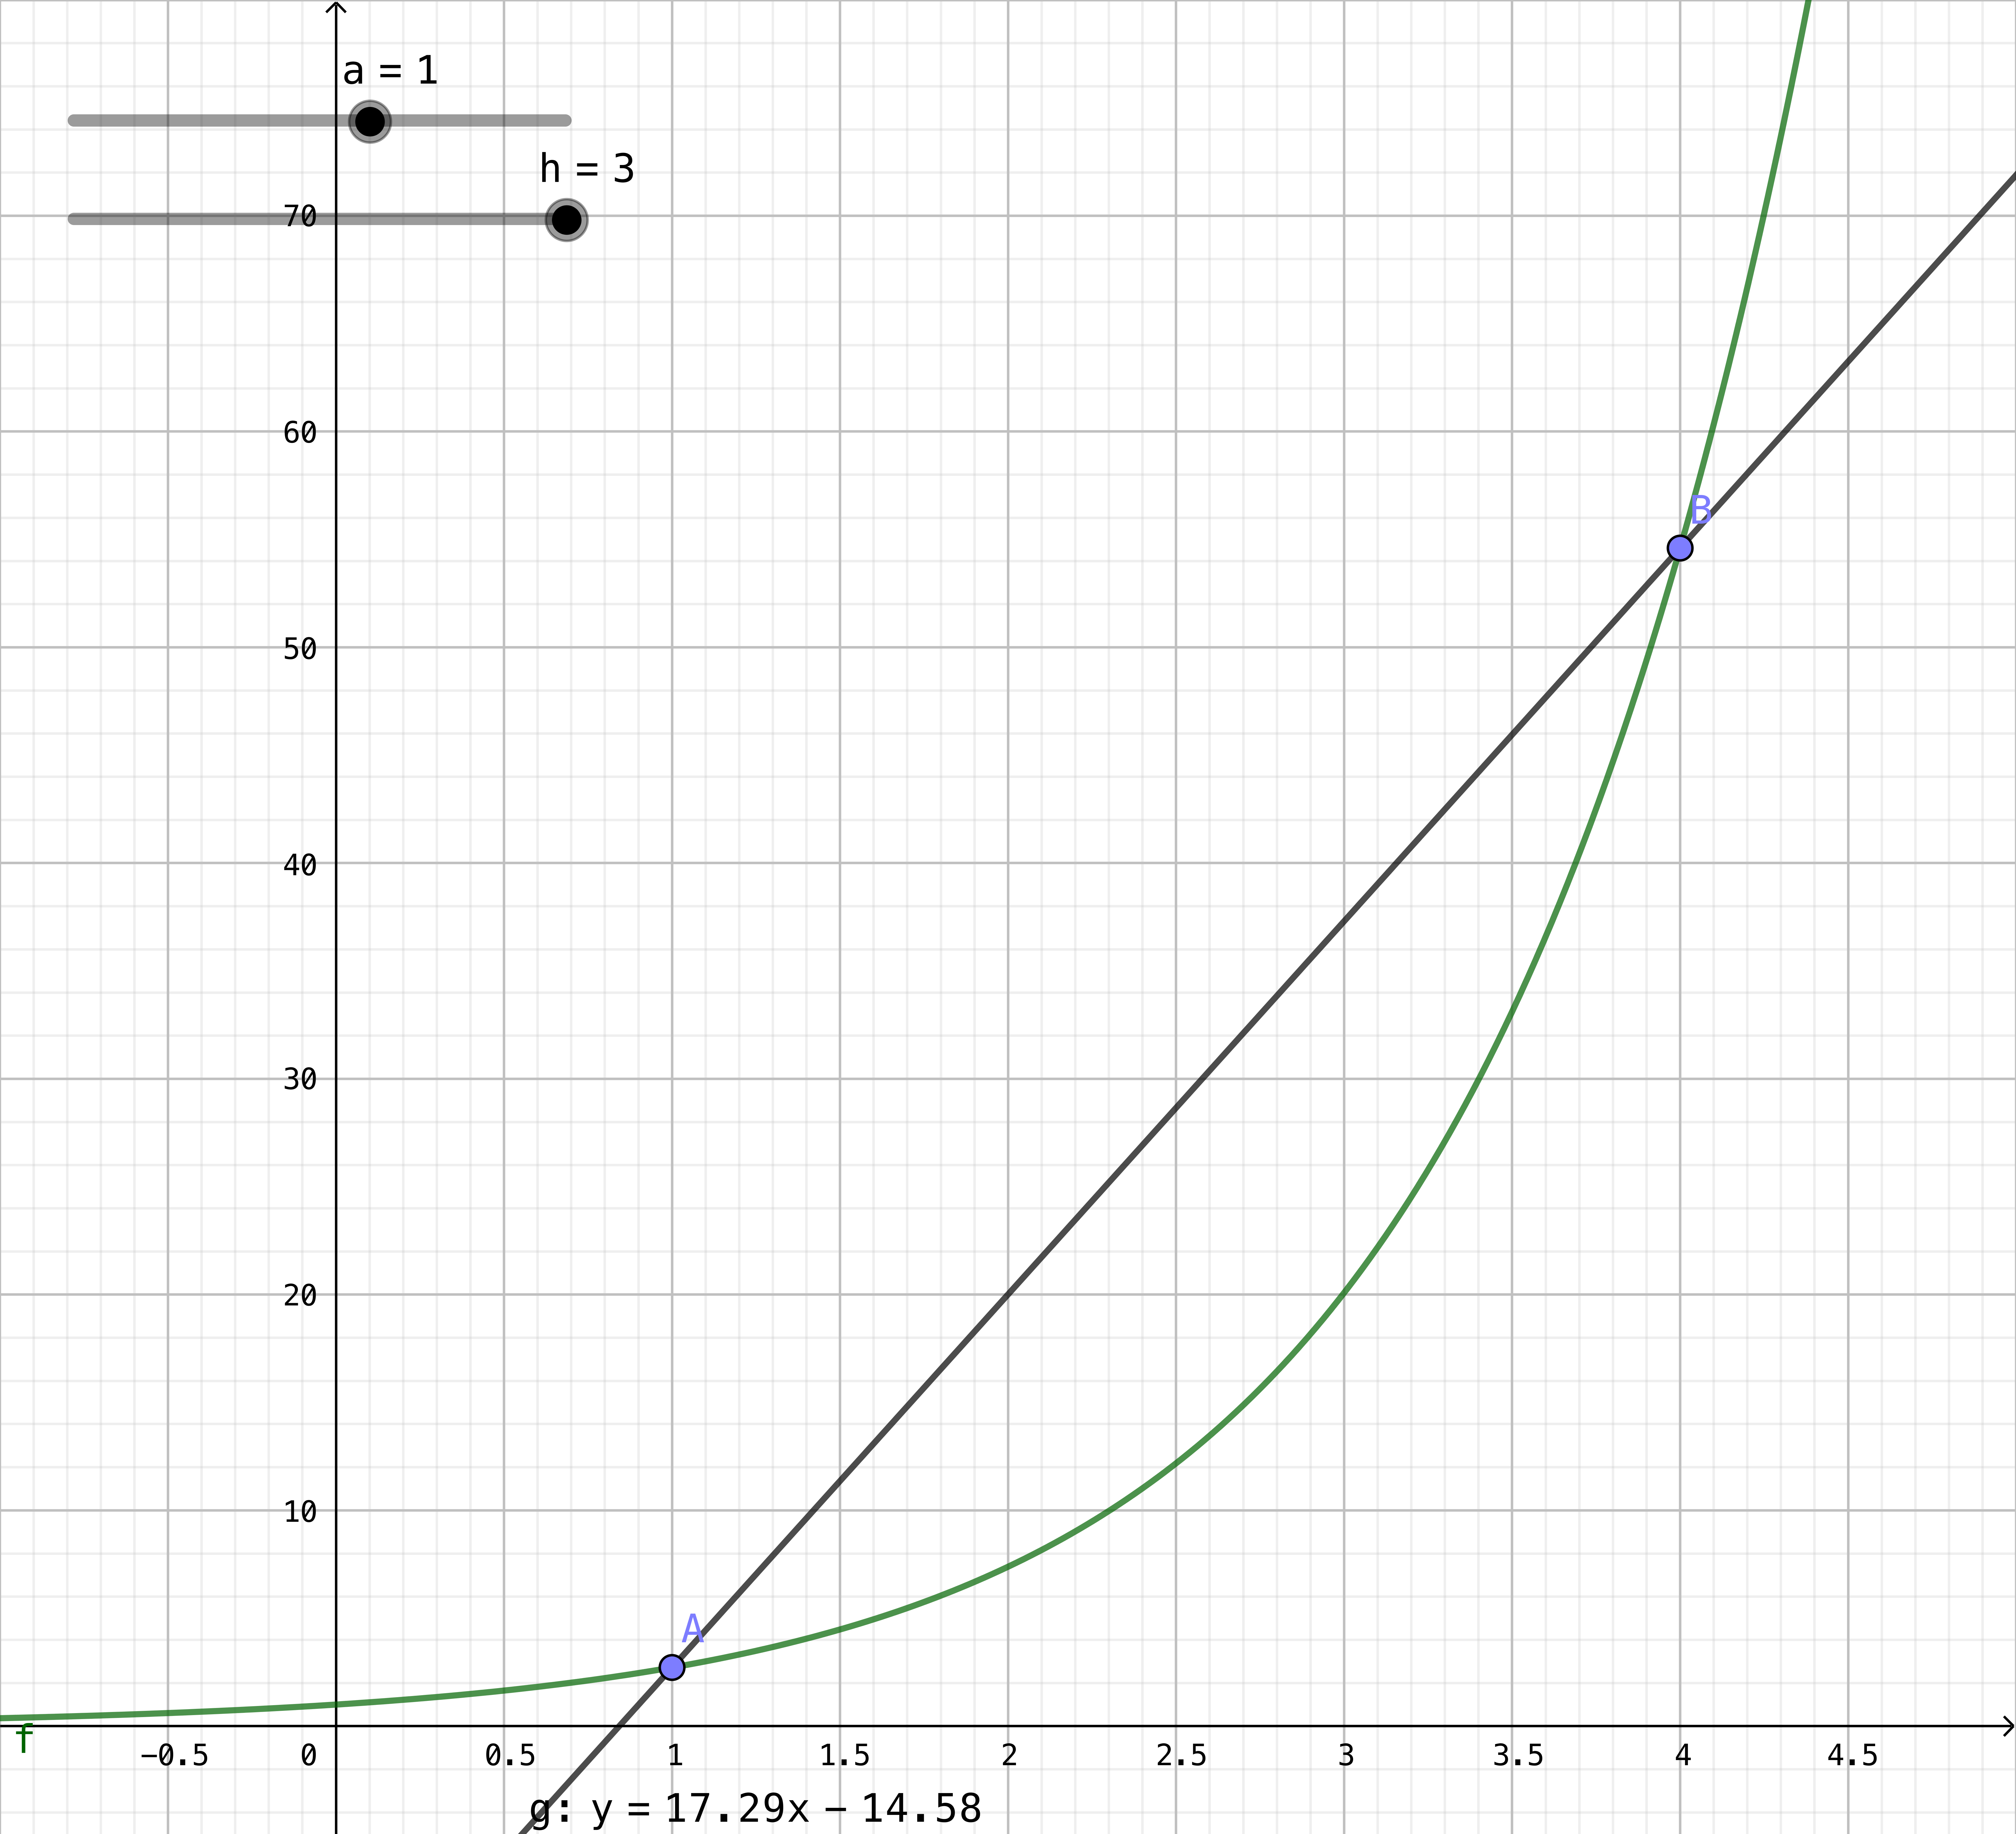
\includegraphics[width=\textwidth]{cl4-8}

\renewcommand\thesubsection{\arabic{subsection}.}
\setcounter{subsection}{9}
\subsection{}
The slope of the secant line between points A and B can
be found using the formula for the Average Rate of Change (ARC),
$$
m = \frac{e^{(a+h)} - e^a}{h} \hspace{6pt}\text{ , here  }\hspace{6pt} m = \frac{e^{4} - e}{3}
$$
\pagebreak

\subsection{}
\emph{Step performed in GeoGebra.}
\\
\\
\textbf{\# 11.} \\
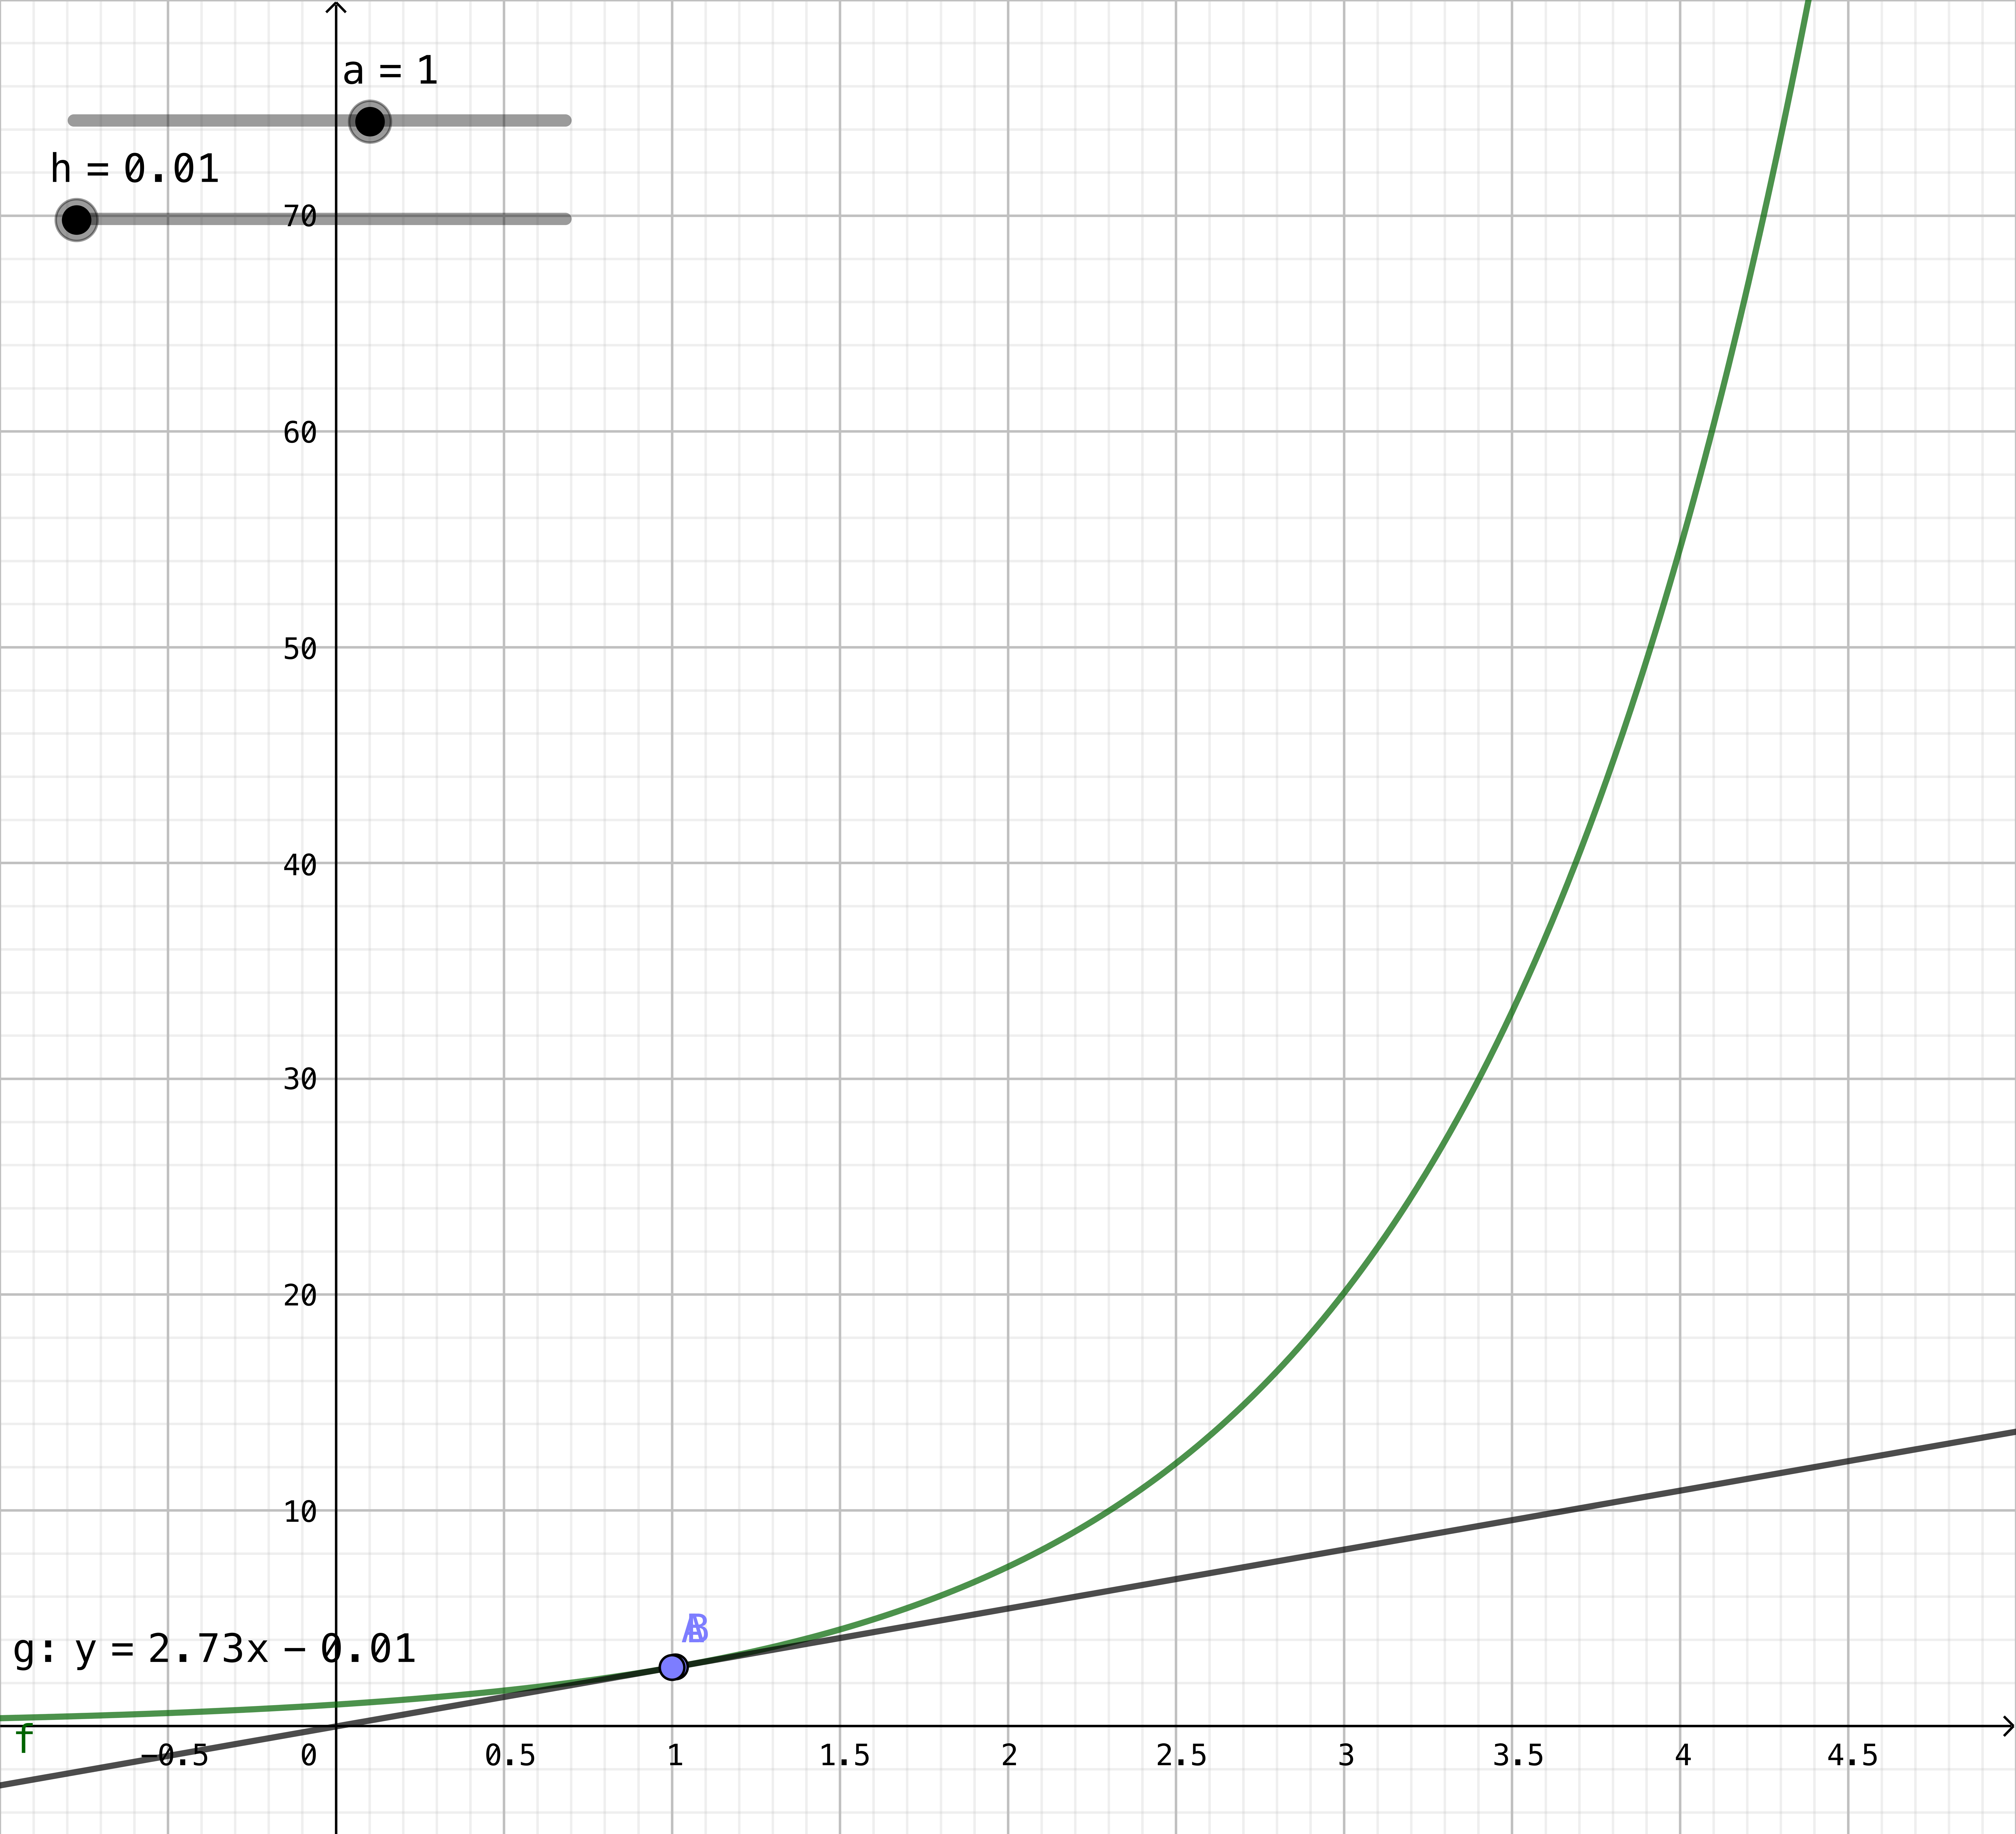
\includegraphics[width=\textwidth]{cl4-11}

\subsection{}
Based on the slope of the line in \# 11, I estimate the slope of the tangent line at point A to be \boxed{\approx 2.73} (which looks a lot like $e$ to me).

\subsection{}
The slope of the tangent is given by the forumla for the Instantaneous Rate of Change (IRC), which is the limit for the expression in \# 10 as the $h$ parameter approaches 0,
$$
m = \lim_{h \rightarrow 0} \frac{e^{(a+h)}-e^{a}}{h} \hspace{6pt}\text{ , here  }\hspace{6pt} m = \lim_{h \rightarrow 0} \frac{e^{(1+h)}-e}{h}
$$

\subsection{}
\emph{Step performed in GeoGebra.}
\\
\\
\textbf{\# 14.} \\
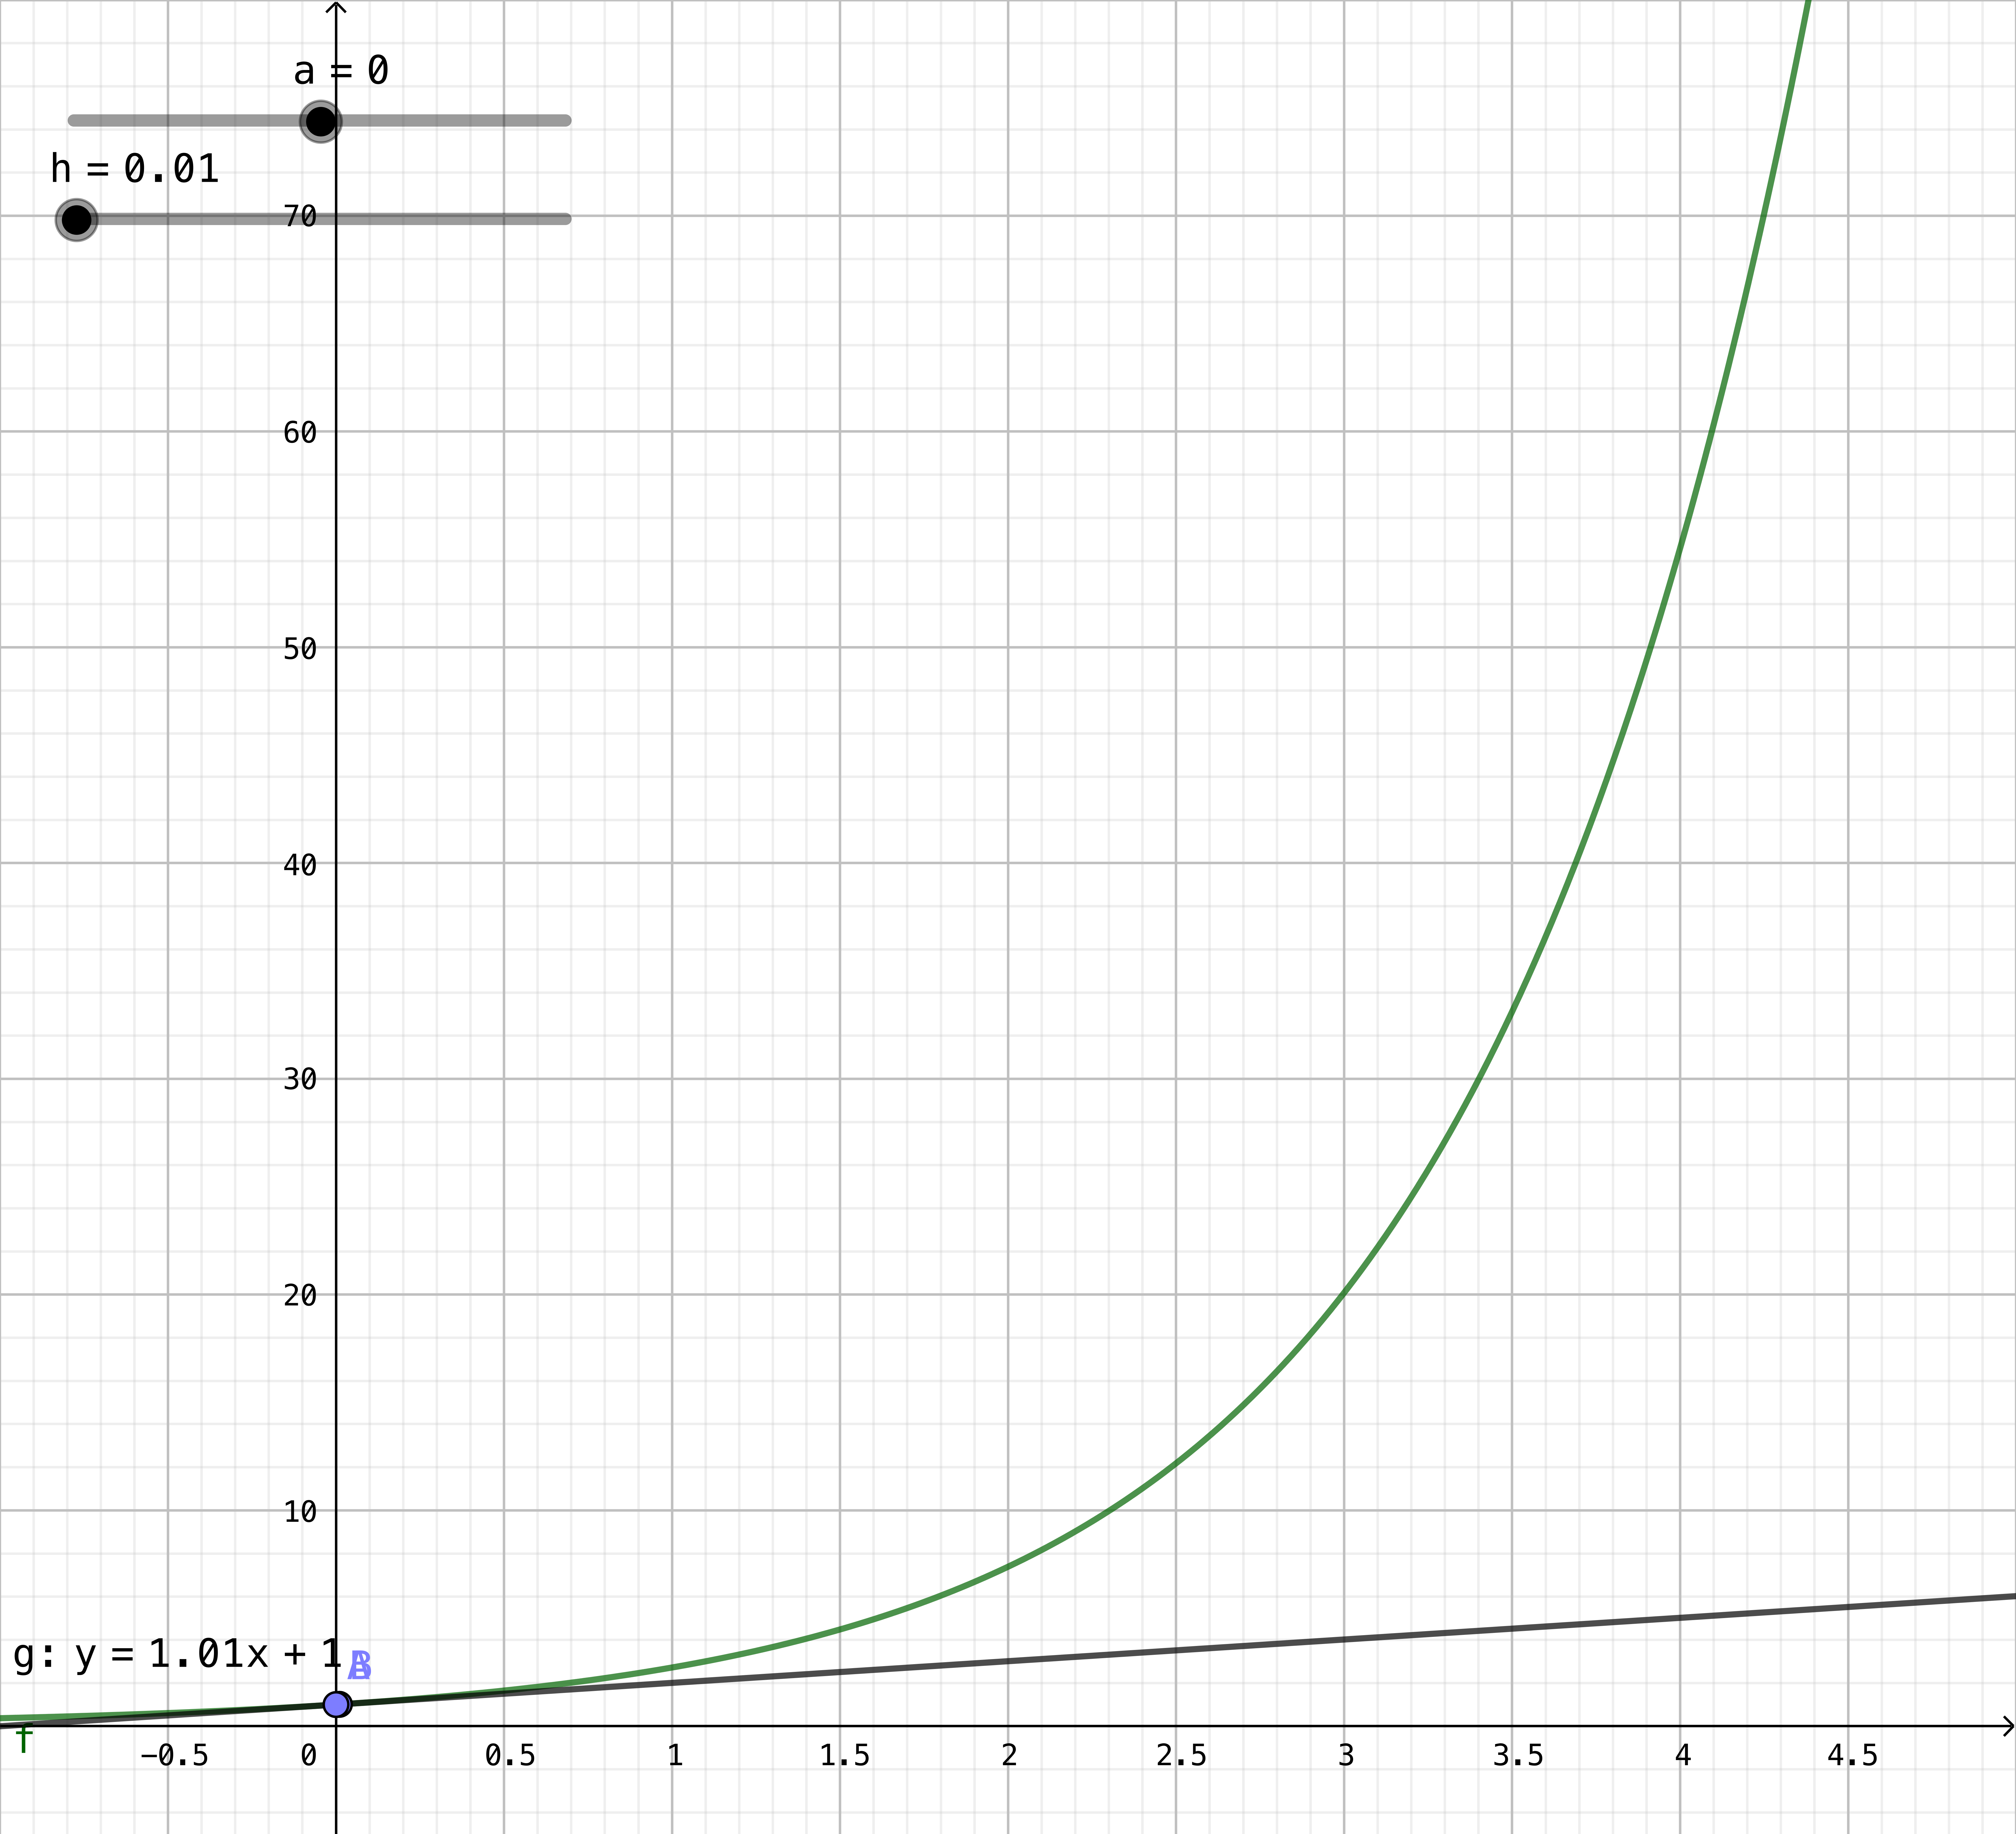
\includegraphics[width=\textwidth]{cl4-14}

The limit expression for the slope of the tangent line of this function at $a=0$ is given by the limit expression
$$
m = \lim_{h \rightarrow 0} \frac{e^{h} - e^0}{h}
$$

By this graphical estimation for a small value of $h=0.01$, the slope of the tangent line at $a=0$ is \boxed{\approx 1.01}.
\end{document}
